\documentclass[legalpaper]{article}
\usepackage{pdflscape}
\usepackage{pgfgantt}
\usepackage{geometry} % to change margins
\usepackage{pdflscape} % provides the landscape environment
\usepackage{ragged2e} % provides \RaggedLeft

\begin{document}

\begin{landscape}
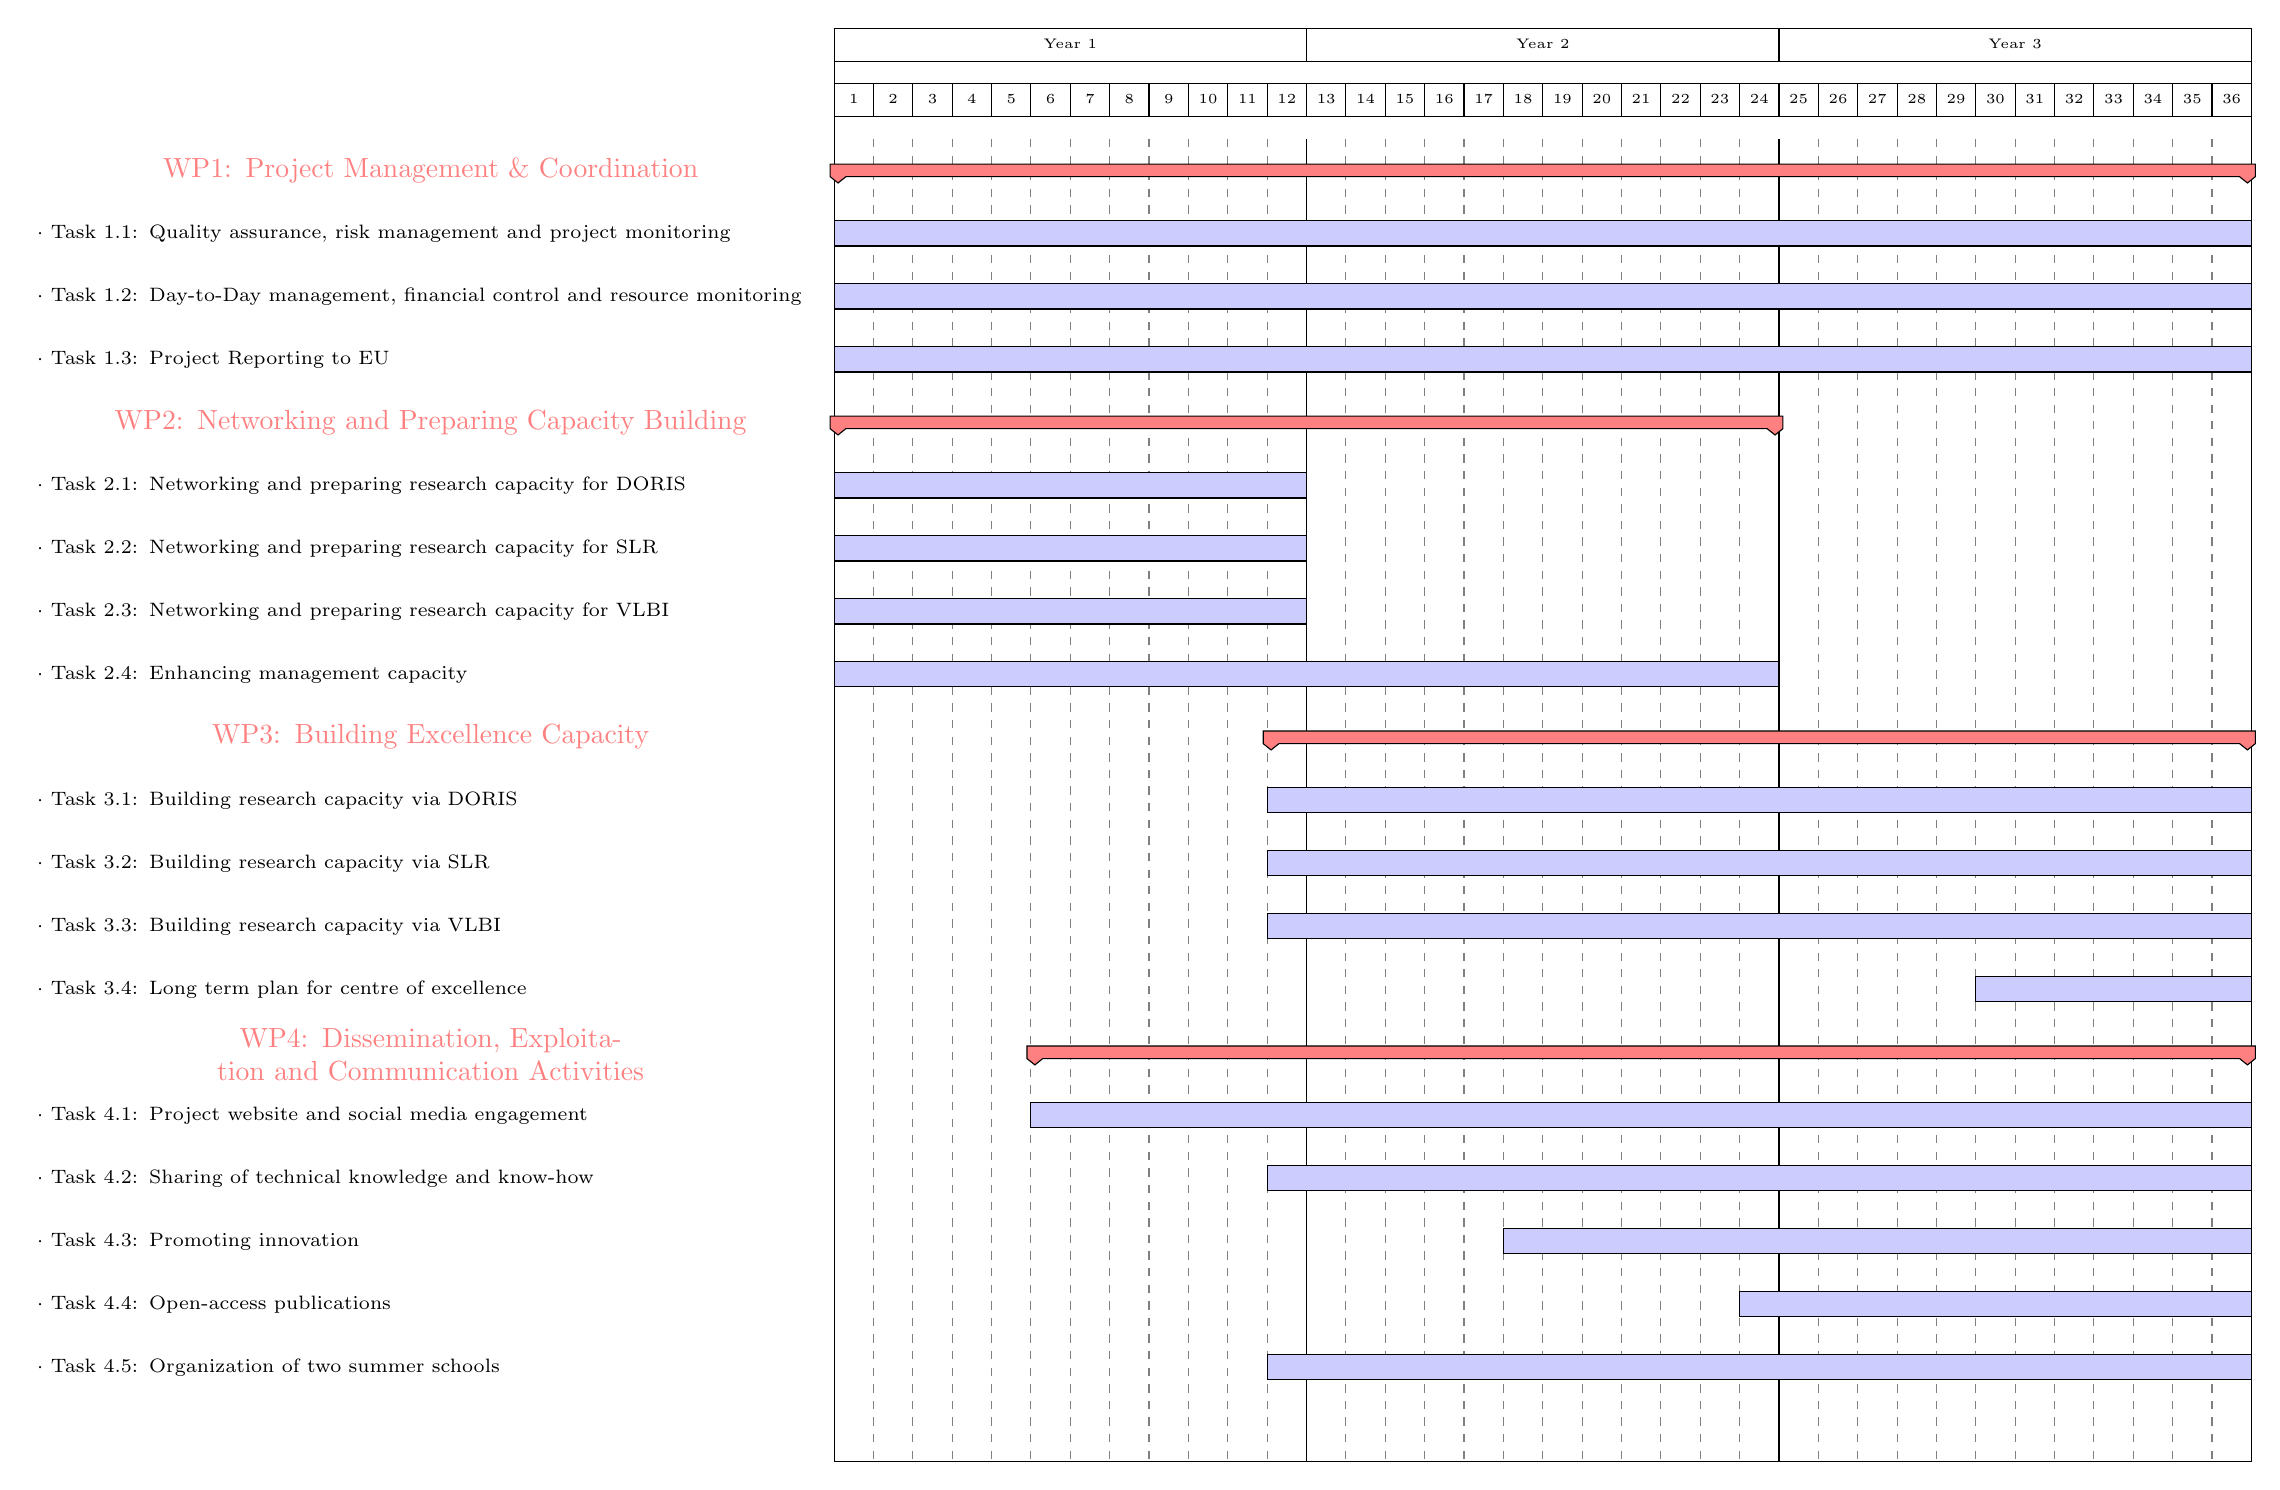
\begin{tikzpicture}
    \begin{ganttchart}[
      y unit chart=.8cm,
      y unit title=.7cm,
      x unit =.5cm,
      vgrid={*{11}{gray, dashed}, *{1}{black}},
      progress label text={\quad\pgfmathprintnumber[precision=0,verbatim]{#1}\%},
      title label font=\tiny,
      group label font=\tiny,
      milestone label font=\tiny,
      group label node/.style={text width=10cm,align=center,font=\color{red!50}\RaggedLeft,anchor=east},
      bar label node/.style={text width=10cm,align=left,font=\scriptsize\RaggedLeft,anchor=east},
      bar label text={$\cdot$ #1},
      milestone inline label node/.append style={left=5mm,font=color{}},
      group/.append style={draw=black, fill=red!50},
      milestone/.append style={fill=orange, rounded corners=2pt},
      bar/.append style={fill=blue!20},
      newline shortcut=true
    ]{1}{36}
    % input years
    \gantttitle{Year 1}{12}
    \gantttitle{Year 2}{12}
    \gantttitle{Year 3}{12} \\
    % input months
    \gantttitlelist{1,...,36}{1} \\
    % WP1
    \ganttgroup{WP1: Project Management \& Coordination}{1}{36} \\
    \ganttbar{Task 1.1: Quality assurance, risk management and project monitoring}{1}{36} \\
    \ganttbar{Task 1.2: Day-to-Day management, financial control and resource monitoring}{1}{36} \\
    \ganttbar{Task 1.3: Project Reporting to EU}{1}{36} \\
    % WP2
    \ganttgroup{WP2: Networking and Preparing Capacity Building}{1}{24} \\
    \ganttbar{Task 2.1: Networking and preparing research capacity for DORIS}{1}{12} \\
    \ganttbar{Task 2.2: Networking and preparing research capacity for SLR}{1}{12} \\
    \ganttbar{Task 2.3: Networking and preparing research capacity for VLBI}{1}{12} \\
    \ganttbar{Task 2.4: Enhancing management capacity}{1}{24} \\
    % WP3
    \ganttgroup{WP3: Building Excellence Capacity}{12}{36} \\
    \ganttbar{Task 3.1: Building research capacity via DORIS}{12}{36} \\
    \ganttbar{Task 3.2: Building research capacity via SLR}{12}{36} \\
    \ganttbar{Task 3.3: Building research capacity via VLBI}{12}{36} \\
    \ganttbar{Task 3.4: Long term plan for centre of excellence}{30}{36} \\
    %\ganttmilestone{Validate usage and manipulation of Earth Orientation Parameters}{9} \\
    %\ganttmilestone{Perform orbit determination via DORIS}{12} \\
    %\ganttmilestone{Perform orbit determination via SLR}{15} \\
    %\ganttmilestone{Incorporate attitude for first satellite, refine to Precise Orbit Determination}{18} \\
    %\ganttmilestone{Consistency between DORIS and SLR}{21} \\
    %\ganttmilestone{Validate estimation of Geodetic Parameters}{24} \\
    %\ganttmilestone{Incorporate attitude for second and third satellites}{30} \\
    % WP4
    \ganttgroup{WP4: Dissemination, Exploitation and Communication Activities}{6}{36} \\
    \ganttbar{Task 4.1: Project website and social media engagement}{6}{36} \\
    \ganttbar{Task 4.2: Sharing of technical knowledge and know-how}{12}{36} \\
    \ganttbar{Task 4.3: Promoting innovation}{18}{36} \\
    \ganttbar{Task 4.4: Open-access publications}{24}{36} \\
    \ganttbar{Task 4.5: Organization of two summer schools}{12}{36} \\
    % bar between Tasks
    %\ganttbar{}{1}{36} \ganttnewline[thick, blue] \\
    %\ganttbar{}{1}{36} \ganttnewline[thick, blue] \\
    %\ganttbar{}{1}{36} \ganttnewline[thick, blue]
    \end{ganttchart}
\end{tikzpicture}
\end{landscape}

\end{document}
